\documentclass[tikz,border=12pt]{standalone}
\usepackage[T1]{fontenc}
\usepackage{mathpazo}
\usepackage{amsmath,amssymb}
\usetikzlibrary{arrows.meta, calc}

\definecolor{stblue}{HTML}{7B97AD}
\definecolor{rwgold}{HTML}{B8995E}
\definecolor{sage}{HTML}{7A9A7E}
\definecolor{dkbrown}{HTML}{3D3530}
\definecolor{wmgray}{HTML}{7B7067}
\definecolor{cream}{HTML}{F9F6F0}
\definecolor{border}{HTML}{D4C9B8}
\definecolor{terracotta}{HTML}{C47A6A}
\definecolor{lavender}{HTML}{907EA0}

\begin{document}
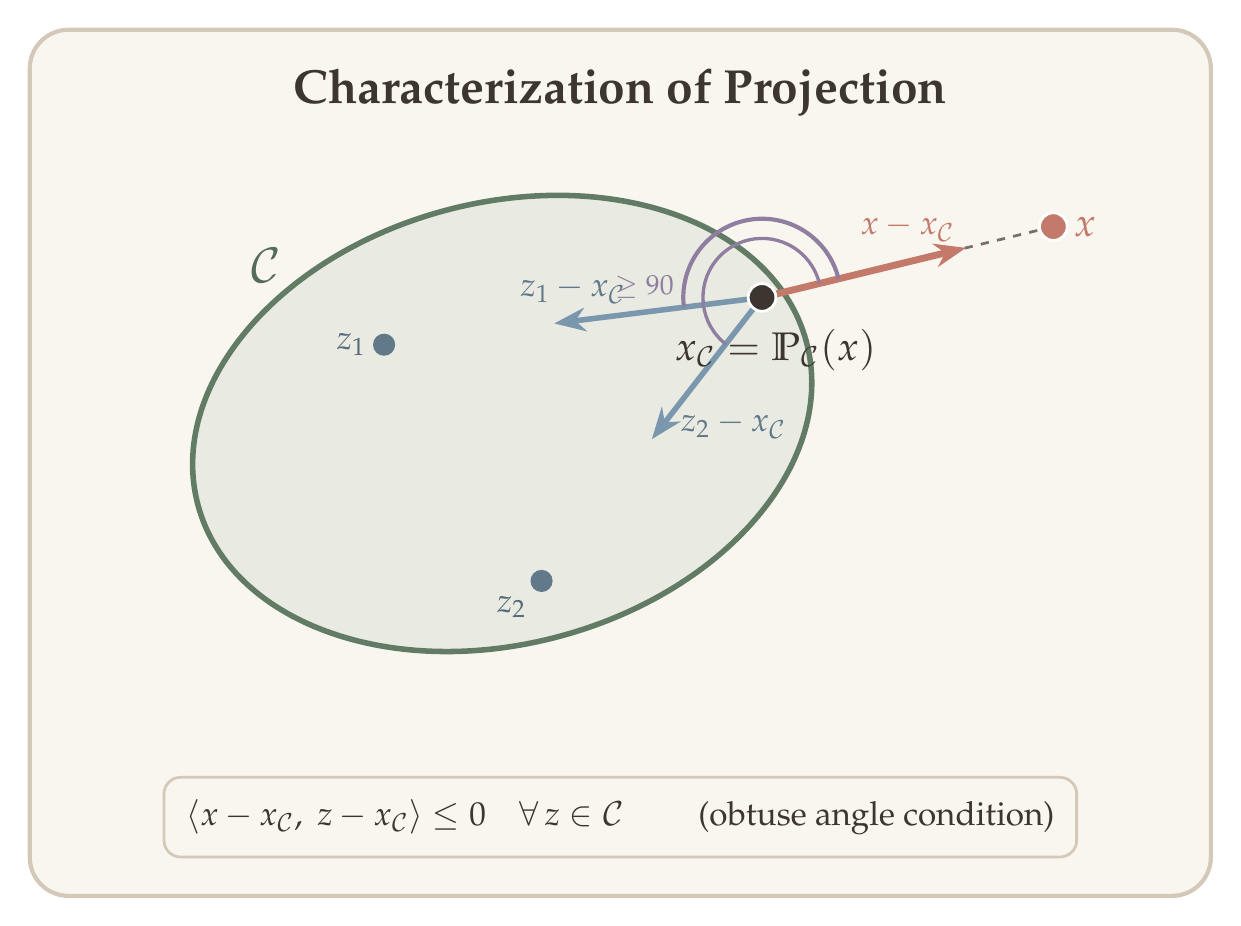
\begin{tikzpicture}[>={Stealth[length=4mm, width=3mm]}]

% Background
\fill[cream, rounded corners=14pt] (-1.5,-2.5) rectangle (13.5,8.5);
\draw[border, line width=1.5pt, rounded corners=14pt] (-1.5,-2.5) rectangle (13.5,8.5);

% Title
\node[text=dkbrown, font=\LARGE\bfseries] at (6.0,7.7)
  {Characterization of Projection};

% Convex set C (tilted ellipse)
\begin{scope}[rotate around={15:(4.5,3.5)}]
  \fill[sage, opacity=0.12] (4.5,3.5) ellipse (4.0cm and 2.8cm);
  \draw[sage!80!black, line width=2pt] (4.5,3.5) ellipse (4.0cm and 2.8cm);
\end{scope}

% Label C
\node[text=sage!70!black, font=\LARGE\bfseries] at (1.5,5.5) {$\mathcal{C}$};

% Key points
\coordinate (x) at (11.5,6.0);       % x outside C
\coordinate (xc) at (7.8,5.1);       % projection on boundary

% Test points inside C
\coordinate (z1) at (3.0,4.5);
\coordinate (z2) at (5.0,1.5);

% --- Dashed line from x to x_C ---
\draw[wmgray, line width=1pt, dashed] (x) -- (xc);

% --- Vector: x - x_C (from x_C toward x) ---
\draw[terracotta, line width=2.5pt, ->]
  (xc) -- ($(xc)!0.7!(x)$);
\node[text=terracotta, font=\large\bfseries, above=4pt]
  at ($(xc)!0.5!(x)$) {$x - x_{\mathcal{C}}$};

% --- Vectors: z - x_C (from x_C toward z_i) ---
\draw[stblue, line width=2pt, ->]
  (xc) -- ($(xc)!0.55!(z1)$);
\node[text=stblue!80!black, font=\large, above=3pt]
  at ($(xc)!0.5!(z1)$) {$z_1 - x_{\mathcal{C}}$};

\draw[stblue, line width=2pt, ->]
  (xc) -- ($(xc)!0.5!(z2)$);
\node[text=stblue!80!black, font=\large, right=3pt]
  at ($(xc)!0.45!(z2)$) {$z_2 - x_{\mathcal{C}}$};

% --- Obtuse angle arc (between x-direction and z1-direction) ---
% Angle from xc to x
\pgfmathanglebetweenpoints{\pgfpointanchor{xc}{center}}{\pgfpointanchor{x}{center}}
\let\angToX\pgfmathresult
% Angle from xc to z1
\pgfmathanglebetweenpoints{\pgfpointanchor{xc}{center}}{\pgfpointanchor{z1}{center}}
\let\angToZone\pgfmathresult
% Angle from xc to z2
\pgfmathanglebetweenpoints{\pgfpointanchor{xc}{center}}{\pgfpointanchor{z2}{center}}
\let\angToZtwo\pgfmathresult

% Arc from z1-direction to x-direction (should span > 90 degrees)
\draw[lavender, line width=1.5pt]
  ($(xc)+({\angToZone}:1.0cm)$) arc[start angle=\angToZone, end angle=\angToX, radius=1.0cm];
\node[text=lavender, font=\normalsize\bfseries] at ($(xc)+(175:1.5cm)$) {$\geq 90°$};

% Arc from z2-direction to x-direction
\draw[lavender, line width=1.2pt]
  ($(xc)+({\angToZtwo}:0.75cm)$) arc[start angle=\angToZtwo, end angle=\angToX, radius=0.75cm];

% --- Points (on top) ---
\fill[terracotta] (x) circle (5pt);
\draw[white, line width=1pt] (x) circle (5pt);
\node[text=terracotta, font=\Large\bfseries, right=4pt] at (x) {$x$};

\fill[dkbrown] (xc) circle (5pt);
\draw[white, line width=1pt] (xc) circle (5pt);
\node[text=dkbrown, font=\Large\bfseries, below=8pt, xshift=5pt] at (xc)
  {$x_{\mathcal{C}} = \mathbb{P}_{\mathcal{C}}(x)$};

\fill[stblue!80!black] (z1) circle (4pt);
\node[text=stblue!70!black, font=\large, left=3pt] at (z1) {$z_1$};
\fill[stblue!80!black] (z2) circle (4pt);
\node[text=stblue!70!black, font=\large, below left=2pt] at (z2) {$z_2$};

% --- Annotation box ---
\node[text=dkbrown, font=\large,
      fill=cream, inner sep=8pt,
      draw=border, line width=1pt, rounded corners=6pt]
  at (6.0,-1.5)
  {$\langle x - x_{\mathcal{C}},\; z - x_{\mathcal{C}} \rangle \leq 0
   \quad \forall\, z \in \mathcal{C}$
   \qquad (obtuse angle condition)};

\end{tikzpicture}
\end{document}
